\chapter{Umsetzung}

Umgesetzt wurde die Aufgabe im wesentlichen aus drei Teilen: 
\begin{itemize}
	\item Einer SQL-Datenbank mit realitätsnahen Tabellen 
	\item Einer Ontologie 
	\item Einem ausführbaren Programm mit Grafischer Benutzungsoberfläche

\end{itemize}

\section{Datenbank}

Bei der Datenbank wurde auf eine gewöhnliche relationale Datenbank zurückgegriffen, da im wesentlichen nur die gängigsten SQL-Befehle benutzt werden. Da es bereits gute Erfahrungen im Team mit MySQL gab, wurde diese Datenbank verwendet. 

Die Datenbank enthält im wesentlichen Informationen die ein Hochschulsportberater ebenfalls nachschlagen würde. Die wichtigsten Informationen sind:
\begin{itemize}
\item angebotene Sportarten
\item Trainingszeiten
\item Veranstaltungsort
\item Höhe der Teilnehmergebühr
\end{itemize} 
Das genaue Datenbankmodell kann der Abbildung \ref{fig:Datenbank-Design} entnommen werden.

\begin{capfigure}[Datenbank-Design]
	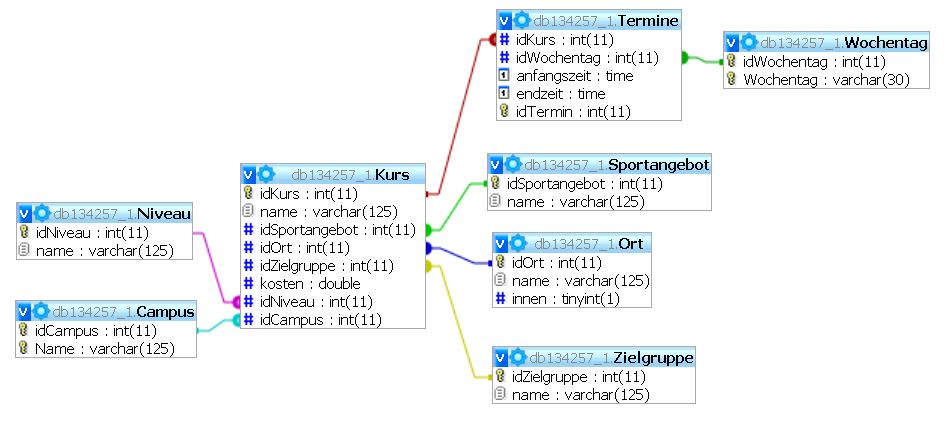
\includegraphics[width=\textwidth]{images/db_design}
\end{capfigure}

\section{Ontologie}
\TODO{[PRIO:SOFORT] Komplett neu machen}
Die Erstellung der Ontologie wird mit \gls{protege} durchgeführt. \gls{protege} ermöglicht nur die Verwendung von OWL-DL. OWL-Full wird nicht unterstützt, daher müssen gewisse Einschränkungen berücksichtigt werden. Beispielsweise kann man keine Komplementklassen erstellen. 

Des Weiteren sollte man immer bedenken, dass eine Ontologie ein Open-World-Szenario darstellt. Im Speziellen kann man nur nach dem Vorhandensein eines Kriteriums abfragen.

Im Laufe dieses Abschnitts wird erläutert, wie die Ontologie erstellt wurde. Im Besonderen werden unsere Entscheidungen bei der Umsetzung begründet und deren Folgen erklärt.

\subsection{Grobe Unterteilung der Ontologie}
Zuerst wird die Klasse \textit{Sport} erstellt. Diese Klasse enthält die beiden Unterklassen \textit{Einzelsport} und \textit{Teamsport}. Da wir uns bei den Sportarten dafür entschieden haben, dass eine Sportart entweder Einzelsport oder Teamsport ist macht diese Unterteilung am meisten Sinn. Natürlich ermöglicht diese Lösung nicht, dass eine Sportart zugleich Einzelsport als auch Teamsport ist. Dies ist aber kein Problem, da es in unserem Szenario nicht vorkommt.

Bei der Darstellung der Ontologie lassen wir die Ebene \textit{Thing} aus Gründen der Übersichtlichkeit weg.
Die Ontologie sieht jetzt wie folgt aus:
\begin{capitemize}[Ontologie - Grober Unterteilung der Ontologie - 1]
		\item Sport
			\begin{itemize}
				\item Einzelsport
				\item Teamsport
			\end{itemize}
\end{capitemize}

Als Nächstes legen wir die Klassen \textit{Ziele} und \textit{Koerperliche\_Einschraenkungen} an. Diese beiden Klassen dienen dazu, die Eigenschaften \textit{Ziele} und \textit{Koerperliche\_Einschraenkungen} abzubilden. Beide Klassen werden noch mit den jeweiligen Unterklassen, die die möglichen Optionen darstellen ergänzt.

Danach sieht die Ontologie wie folgt aus:
\begin{capitemize}[Ontologie - Grober Unterteilung der Ontologie - 2]
	\item Koerperliche\_Einschraenkungen
		\begin{itemize}
				\item Armbereich
				\item Beinbereich
				\item Hoehenangst
		\end{itemize}
	\item Sport
		\begin{itemize}
			\item Einzelsport
			\item Teamsport
		\end{itemize}
	\item Ziele
		\begin{itemize}
				\item Fitness
				\item Freizeitvergnuegen
				\item SelfDefense
				\item Sozialkontakte
				\item Wettbewerb
		\end{itemize}
\end{capitemize}

Damit sind die Klassen soweit fertig. Beide Klassen wurden in dieser Art angelegt, da sie optional sind. Ein Sport muss keine Verknüpfung zu diesen Klassen haben. Jetzt werden noch die Object Properties dazu wie folgt angelegt:

\begin{capitemize}[Properties - hatZiel und ungeeignetBei]
	\item hatZiel
		\begin{itemize}
			\item Domains: \textit{Sport}
			\item Ranges: \textit{Ziele}
		\end{itemize}
	\item ungeeignetBei
		\begin{itemize}
			\item Domains: \textit{Sport}
			\item Ranges: \textit{Koerperliche\_Einschraenkungen}
		\end{itemize}
\end{capitemize}

Nun lassen sich die Ziele und Einschränkungen mit den Sportarten verbinden. Ein Problem ergibt sich mit dieser Variante allerdings noch, man kann nicht nach Sportarten suchen die explizit keine Einschränkungen haben. Bei den Zielen gibt es die gleiche Einschränkung, allerdings ist sie dort egal, da eine Suche nach Sportarten, die explizit keine Ziele haben keinen Sinn ergibt. Bei den Einschränkungen muss allerdings eine Lösung her. Da in einem Open-World-Szenario nur nach dem Vorhandensein gefragt werden kann, haben wir uns dazu entschieden noch die Unterklasse \textit{Keine} bei den Körperlichen Einschränkungen zu ergänzen. Jetzt hat man die Möglichkeit, auch Sportarten zu suchen, die bei keiner Einschränkung ungeeignet sind.

Bei den Sportarten muss jetzt jede Sportart die Object Property \textit{ungeeignetBei} verwenden. Für die Object Property \textit{hatZiel} gilt das nicht.

\TODO{istExotisch, istKampfsport, istKoerperkontakt, istWassersport - Problem erw\"ahnen, dass man nicht nach Boolean abfragen kann}

\TODO{Klasse Boolean als L\"osung f\"ur das Problem}

\TODO{\"Aquivalenzklassen, Aufbau einer Sportart, etc.}

\section{Programm}

Dieser Abschnitt geht zuerst auf die Entscheidung zum Aufbau der graphischen Oberfläche ein und behandelt danach die technischen Aspekte des Programms. 

\subsection{Entscheidung zum Aufbau der graphischen Oberfläche}
Bei der Gestaltung der GUI, wurde sich dafür entschieden, dass der Benutzer zu jedem Zeitpunkt möglichst alle Auswahlmöglichkeiten vor Augen hat und dass er, ebenfalls zu jedem Zeitpunkt, eine Liste mit den Sportarten erhalten kann, die zu seinen Auswahlkriterien passen.

Die Gründe für diese Entscheidungen sind zum einen die Benutzerfreundlichkeit. Durch diesen Aufbau soll der Benutzer aufgefordert werden, möglichst viele Auswahlkriterien auszuprobieren, da er sofort testen kann, welche Auswirkungen diese auf die Auswahl der Sportarten hat. Dies hat den Vorteil, dass der Benutzer die Kriterien mit, einer für ihn, hohen Priorität setzen kann und unangerührt lässt, währendem er die Kriterien mit einer, für ihn, niedrigen Priorität schnell und einfach ändern kann. Ein konkretes Beispiel hierfür wäre z.B. die Sportart Klettern. Für einige Benutzer ist die Höhenangst nur ein leichtes Problem, für einige andere ist sie unüberwindlich. Somit haben die Benutzer mit leichter Höhenangst, die Möglichkeit die angebotenen Sportarten mit oder ohne Höhenangst zu vergleichen, während jene mit starker Höhenangst das Kriterium auswählen und nicht mehr deaktivieren.

Ein anderer Grund für diese Entscheidung war die Tatsache, dass unsere Szenarien wenige Sprünge von einem Schritt zu einem anderen beinhalten. Deshalb haben wir uns dagegen entschieden eine Frage nach der anderen abzuhandeln, wie die Szenarien dies eigentlich vorsehen und bei mehreren Sprüngen wohl auch einfacher umzusetzen gewesen wäre. Nichtsdestotrotz wird am Ende dieses Abschnittes erläutert wie mehrere dieser Sprünge dargestellt werden könnten, obwohl der Benutzer nach wie vor sämtliche Optionen vor Augen hat und möglichst wenig an Flexibilität einbüßt.
\TODO{richtige referenz setzen}

\subsection{Aufbau der graphischen Oberfläche}

Bei der Abbildung \ref{fig:Hauptfenster} handelt es sich um das Hauptfenster, in dem der Benutzer die Möglichkeit hat seine Auswahlkriterien festzulegen, die Suche zu starten sowie die vorgeschlagen Sportarten einzusehen und Informationen über diese zu erhalten. Bei den Auswahlkriterien handelt es sich um jene, die benötigt werden, um die Fragen aus den Szenarien zu beantworten.

Bei der Abbildung \ref{fig:Auswahl der Zeiten} handelt es sich um einen "`Stundenplan"', in dem der Benutzer die Zeiträume festlegen kann, in denen er wöchentlich Sport treiben will. 

%\begin{capfigure}[Hauptfenster]%
%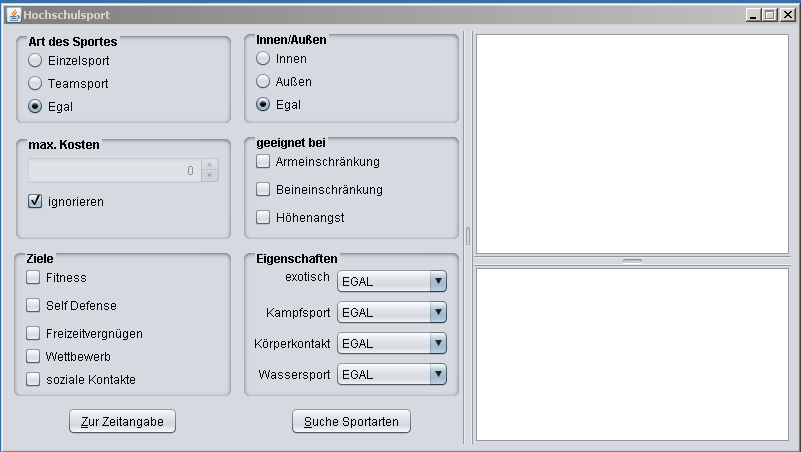
\includegraphics[width=\textwidth]{images/gui.png}%
%\end{capfigure}

%\begin{capfigure}[Auswahl der Zeiten]%
%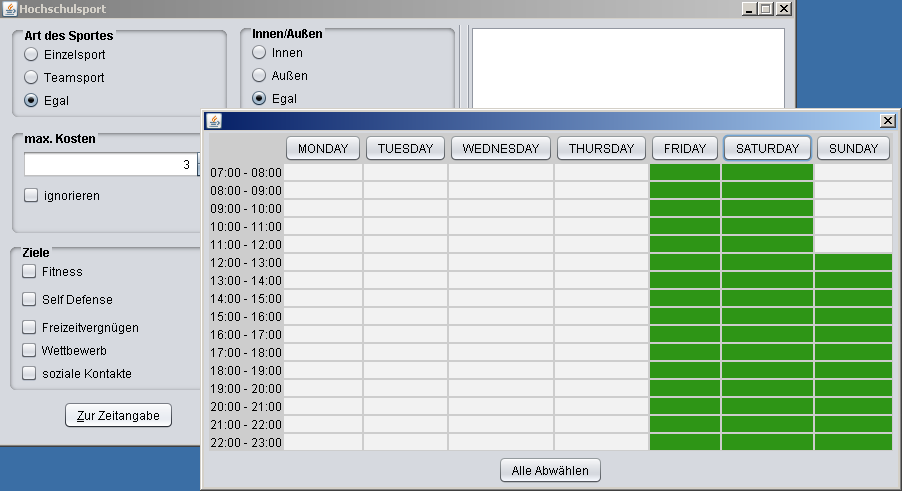
\includegraphics[width=\textwidth]{images/guizeit.png}%
%\end{capfigure}

\begin{figure}[p]
\centering
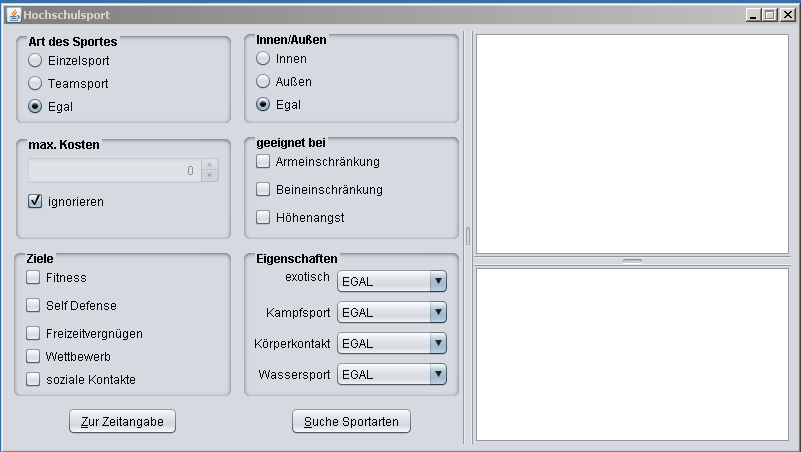
\includegraphics[width=\textwidth]{images/gui.png}%
\caption{Hauptfenster}
\label{fig:Hauptfenster}
\end{figure}

\begin{figure}[p]
\centering
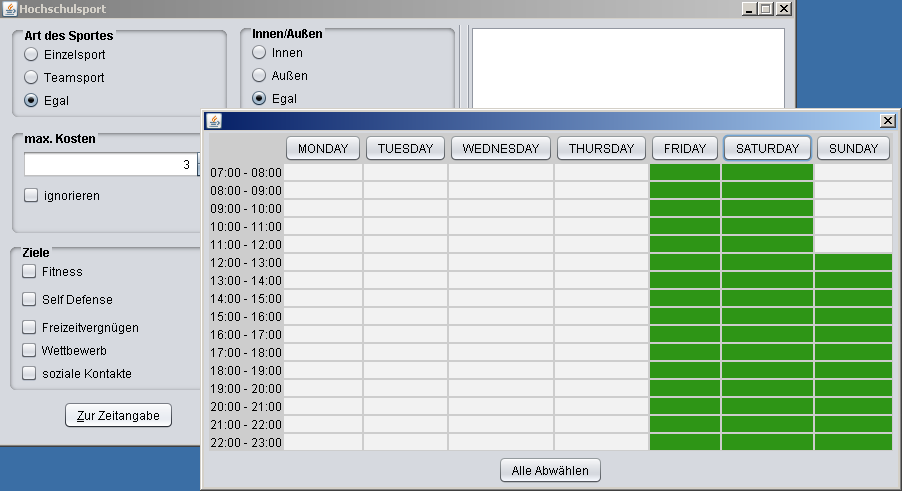
\includegraphics[width=\textwidth]{images/guizeit.png}%
\caption{Auswahl der Zeiten}
\label{fig:Auswahl der Zeiten}
\end{figure}

\subsection{Technische Umsetzung}
Das Programm wurde mit Java geschrieben und benutzt die Semantic Web OWL API \autocite{semweb:owlapi} als Verbindung zur Ontologie. Beim benutzten Reasoner handelt es sich um HermIT\autocite{krr:hermit}. Die Verbindung zur Datenbank wird durch einen JDBC-Treiber\autocite{oracle:jdbc} realisiert.

Beim Ausführen der Suche wird zunächst eine Menge mit sämtlichen verfügbaren Sportarten erstellt, die daraufhin nach Bedarf gefiltert wird. Der Einfachheit halber wird für jedes Auswahlkriterium, falls dieses nicht ignoriert werden soll, eine Query ausgeführt, die die Menge mit den Sportarten weiter filtert. Jede Query hat folgenden, gleichen Aufbau\footnote{UML angelehnte Schreibweise \lstinline"  operation(arg list) : return type" \autocite{kow:umlclass}} \lstinline"query(Sportarten) : gefilterte_Sportarten". Dies bedeutet, dass eine Query eine Menge von Sportarten enthält und nach einem bestimmten Auswahlkriterium filtert, um dann die gefilterte Menge zurückzugeben. Durch den jeweils gleichen Aufbau ergibt sich der Vorteil, dass die Reihenfolge der Queries keine Rolle spielt, und sie demnach auch bei Bedarf übersprungen werden können. Das Überspringen von Queries wird benötigt, da jedes Auswahlkriterium vom Benutzer ignoriert werden kann und somit keinen Einfluss auf den Auswahlprozess nimmt.

Das Listing \ref{lst:filtern} zeigt das Filtern an einem konkreten Beispiel. In einem ersten Schritt werden die Sportarten abgefragt. Danach werden die einzelnen Queries durchlaufen, wobei immer abgefragt wird, ob das entsprechende Auswahlkriterium nicht ignoriert werden soll. Im Beispiel wird der nach dem maximalen Preis und den Zielen gefiltert. Es sei noch darauf hingewiesen, dass es an dieser Stelle im Code keinen Unterschied macht, ob die Query über die Datenbank (für den Preis) oder die Ontologie (für die Ziele) ausgeführt wird. 

\begin{lstlisting}[float=htbp, caption=Filtern von Sportarten, label=lst:filtern]
Set<Sportangebot> sport = Queries.querySport();
...        
if (!ignorePrice) {
	sport = Queries.queryPrice(sport, maximalPrice);
}
...
if (ziele.length > 0) {
	//der Benutzer hat Ziele ausgewaehlt
	sport = Queries.queryZiele(sport, ziele);
}
...                
\end{lstlisting}

\section{Realisierung der Sprünge}
Da es in unseren Szenarien nur wenige Sprünge gibt, wurde deren Logik fest in die GUI hinein programmiert. Die einzelnen Sprünge sind im folgenden aufgelistet und es wird beschrieben, wie diese umgesetzt wurden.

\subparagraph{Überspringen einzelner Fragen.} Der Benutzer kann in der GUI bei verschiedenen Fragen "`Egal"' auswählen, so dass diese nicht in Betracht gezogen werden. 
\subparagraph{Die Frage ob das Sportangebot etwas kosten darf.} Der Benutzer hat hier die Möglichkeit, die Frage zu ignorieren, oder einen maximal Preis anzugeben.
\subparagraph{Hat der Benutzer eine Einschränkung, so darf beim Sportangebot kein Körperkontakt bestehen.} Wählt der Benutzer eine Einschränkung, so wird die Auswahlmöglichkeit zum Körperkontakt automatisch auf "`Nein"' gestellt und er kann diese Auswahl nicht mehr ändern. Es sei denn er wählt sämtliche Einschränkungen wieder ab.
\subparagraph{Sprung zu einer beliebigen Frage.} Da der Benutzer sämtliche Auswahlkriterien zu jedem Zeitpunkt sehen kann, ist dieser Sprung nicht relevant.

\subsection{Realisierung von mehreren Sprüngen}
Die zuvor genannte Vorgehensweise ist recht gut geeignet, falls die Szenarien nur wenige Sprüngen enthalten. Ab einer bestimmten Zahl solcher Sprünge braucht man eine andere Vorgehensweise, bei der diese nicht mehr hart-codiert sind, sondern möglichst dynamisch verändert werden können.

Eine Idee wäre es verschiedene Personenarten in die Ontologie einzuführen. Je nach dem welche Angaben der Benutzer ausgewählt hat, ermittelt die Ontologie um welche Art von Person es sich beim Benutzer handelt. Die GUI erhält die Personenart und kann entsprechend darauf reagieren, indem sie z.B. verschiedene Felder automatisch auswählt, hervorhebt oder versteckt.

Als Beispiel könnte man eine Personenart \lstinline"eingeschraenkte_Person" in der Ontologie einführen, die eine Unterklasse von \lstinline"Person" ist und als Property \lstinline"hat_Einschraenkung some koerperliche_Einschraenkung" besitzt. Wählt der Benutzer nun als körperliche Einschränkung den Beinbereich aus, so wird eine Query an die Ontologie abgesetzt, die wie folgt aussieht: \lstinline"Person and hat_Einschraenkung some Beinbereich", das Ergebnis dieser Query wäre die Klasse \lstinline"eingeschraenkte_Person". Da die GUI nun weiß, dass es sich beim Benutzer um eine \lstinline"eingeschraenkte_Person" handelt, kann die Auswahloption der Kampfsportart, wie im Szenario beschrieben, auf \lstinline"Nein" gesetzt werden.

Das Beispiel kann wie folgt erweitert werden: führt man eine weitere Personenart \lstinline"zahlende_Person" mit der Property \lstinline"will_zahlen only True", wobei es sich bei dem True um einen von uns eingeführten Boolean Wert handelt. Dies ermöglicht es folgende Query abzusetzen: \lstinline"Person and (hat_Einschraenkung some Beinbereich or will_zahlen only True)". Das Ergebnis sind folgende Personenarten: \lstinline"eingeschraenkte_Person, zahlende_Person". Die GUI kann daraufhin auf die einzelnen Personenarten reagieren und wie oben beschrieben ihr Aussehen ändern. Ein Vorteil dieser Methode ist, dass man die Query beliebig mit der Oder-Verknüpfung erweitern kann, so dass man bei Bedarf weitere Kriterien aufnehmen kann.

In diesem Beispiel müssen zwei unabhängige Teile der GUI verändert werden, es ist jedoch vorstellbar, dass es Personenarten gibt, die gleichzeitig auftreten können, allerdings widersprüchliche Effekte in der GUI auslösen sollen. So könnte z.B. ein bestimmtes Feld für die eine Personenart aus- und für die andere Personenart angeschaltet werden. Wie solche Konflikte zu lösen sind, hängt von den konkreten Fällen ab. Ein möglicher Lösungsansatz wäre aber ein Priorisieren der verschiedenen Personenarten. Dies bedeutet, dass sich die Personenart mit der höheren Priorität durchsetzt und die GUI deren Effekte übernimmt. Die Prioritäten könnten auch vom Benutzer mitbestimmt werden, indem er festlegen kann, wie wichtig ihm verschiedene Auswahlkriterien sind.

\TODO{[PRIO:NORMAL]fÜr Gilles: beschreibe einzelne Fragen mit CardLayout}